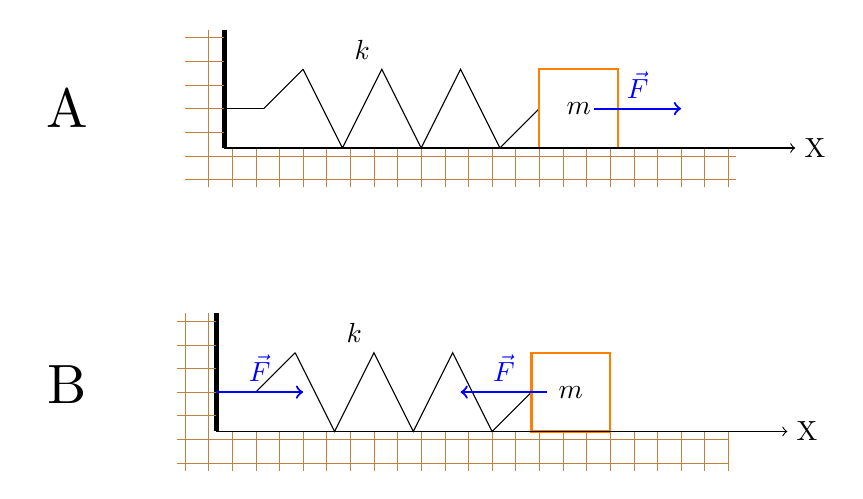
\begin{tikzpicture}
%primer dibujo
\draw [ultra thick](-1,1) -- (-1,-0.5);
\draw (-1,0) -- (-0.5,0) node (v1) {};
\draw (0,0.5) node (v2) {} -- (0.5,-0.5) -- (1,0.5) -- (1.5,-0.5) -- (2,0.5) -- (2.5,-0.5) -- (3,0);
\draw (v1.center) -- (v2.center);

\node at (3.5,0) {$m$};
\draw [brown](-1,-0.5) node (v4) {} -- (5.5,-0.5);

\draw [help lines, step=0.3cm, brown] (-1.5,-1) grid (-1,1);
\draw [help lines, step=0.3cm,brown] (-1,-1) grid (5.5,-0.5) node (v3) {};

\draw  [orange, thick](3,0.5) rectangle (4,-0.5);
\draw [->](v4.center) -- (6.25,-0.5);
\node at (6.5,-0.5) {X};
\node at (0.75,0.75) {$k$};
\draw [thick, blue, ->](3.7,0) -- (4.8,0) node [midway, above]{$\vec{F}$};

%segundo dibujo
\draw [ultra thick](-1.1,-2.6) -- (-1.1,-4.1);
\draw (-1.1,-3.6) -- (-0.6,-3.6) node (v1) {};
\draw (-0.1,-3.1) node (v2) {} -- (0.4,-4.1) -- (0.9,-3.1) -- (1.4,-4.1) -- (1.9,-3.1) -- (2.4,-4.1) -- (2.9,-3.6);
\draw (v1.center) -- (v2.center);

\node at (3.4,-3.6) {$m$};
\draw [brown](-1.1,-4.1) node (v4) {} -- (5.4,-4.1);

\draw [help lines, step=0.3cm, brown] (-1.6,-4.6) grid (-1.1,-2.6);
\draw [help lines, step=0.3cm,brown] (-1.1,-4.6) grid (5.4,-4.1) node (v3) {};

\draw  [orange, thick](2.9,-3.1) rectangle (3.9,-4.1);
\draw [->](v4.center) -- (6.15,-4.1);
\node at (6.4,-4.1) {X};
\node at (0.65,-2.85) {$k$};
\draw [thick, blue, <-](2,-3.6) -- (3.1,-3.6) node [midway, above]{$\vec{F}$};


\node at (-3,0) [scale=2]{A};
\node at (-3,-3.5) [scale=2]{B};
\draw [thick, blue, ->](-1.1,-3.6) -- (0,-3.6) node [midway, above]{$\vec{F}$};
\end{tikzpicture}